\documentclass[11pt]{article}
\usepackage{epsf,amsmath,amsfonts,amsthm,graphicx,color}
%\usepackage{draftcopy}
\textwidth=7in
\textheight=9.0in
\hoffset=-1in
\voffset=-1in
\bibliographystyle{alpha}

\usepackage{amsthm, amsmath, amssymb, amsfonts, graphicx, graphics,epsfig, bbm, xcolor, hyperref,subfigure,float}


\newcommand{\xinnote}[1]{ {\textcolor{red}  {\mbox{**Xin:} #1}}}
\newcommand{\nichollsnote}[1]{ {\textcolor{yellow}  {\mbox{**Nicholls:} #1}}}
\newcommand{\hpra}{\frac{H_p^{(1)}(kr)}{H_p^{(1)}(ka)} }
\newcommand{\hprb}{\frac{H_p^{(1)}(kr)}{H_p^{(1)}(kb)} }
\newcommand{\diffhpn}{\frac{d_z^nH_p^{(1)}(ka)}{H_p^{(1)}(ka)} }
\newcommand{\diffhpnm}{\frac{d_z^{n-m}H_p^{(1)}(ka)}{H_p^{(1)}(ka)} }
\newcommand{\ep}{e^{ip\theta}}
\newcommand{\opD}{\mathcal{D}}
\newcommand{\jpra}{\frac{J_p(kr)}{J_p(ka)} }
\newcommand{\diffjpn}{\frac{d_z^nJ_p(ka)}{J_p(ka)} }
\newcommand{\diffjpnm}{\frac{d_z^{n-m}J_p(ka)}{J_p(ka)} }

\begin{document}
\noindent\textbf{\large LGSPR  with (ALMA), vacuum and vacuum, $\exp(\cos)$, $\bar{g} = 0.025, 0.05, 0.5, 1$}
\begin{figure}[H]
	\centering
	\subfigure
	{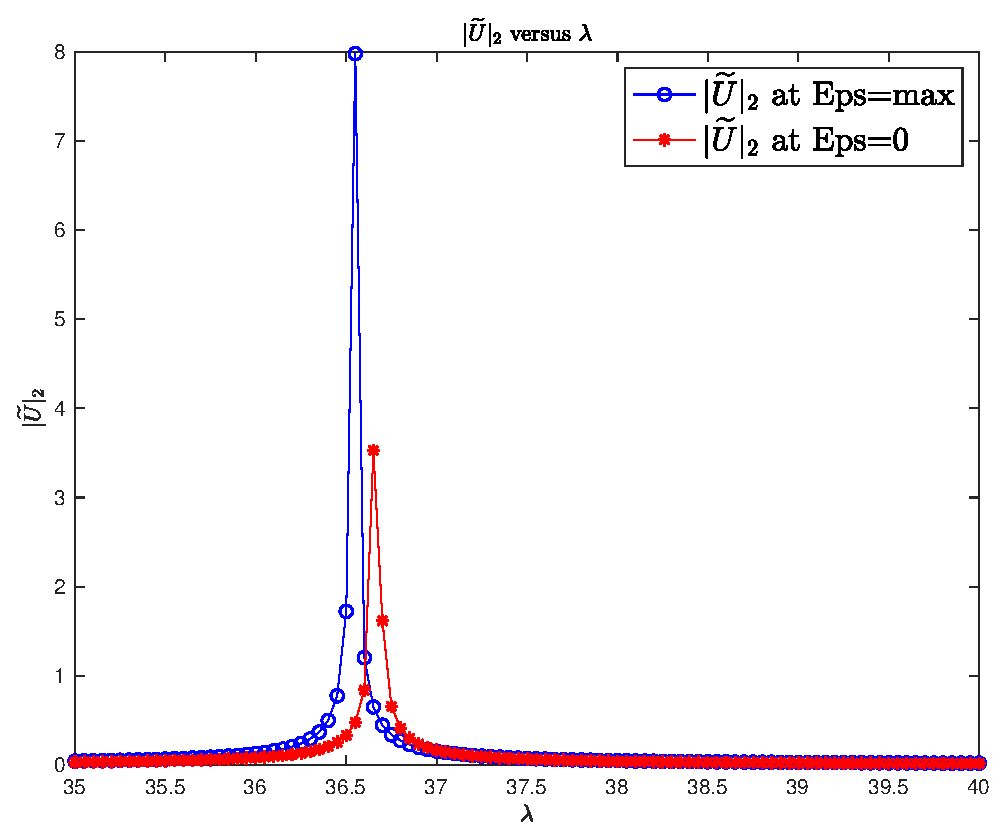
\includegraphics[width=0.35\textwidth]
		{fig_LGSPR_GU_shift_expcos_gbar25_VACUUM.pdf}}
	\quad
	\subfigure 
	{\includegraphics[width=0.35\textwidth]
		{fig_LGSPR_GW_shift_expcos_gbar25_VACUUM.pdf}}
	\\
	\subfigure
	{\includegraphics[width=0.35\textwidth]
		{fig_LGSPR_GU_shift_expcos_gbar50_VACUUM.pdf}}
	\quad
	\subfigure
	{\includegraphics[width=0.35\textwidth]
		{fig_LGSPR_GW_shift_expcos_gbar50_VACUUM.pdf}}
	\\
	\subfigure 
	{\includegraphics[width=0.35\textwidth]
		{fig_LGSPR_GU_shift_expcos_gbar500_VACUUM.pdf}}
	\quad
	\subfigure 
	{\includegraphics[width=0.35\textwidth]
		{fig_LGSPR_GW_shift_expcos_gbar500_VACUUM.pdf}}
	\\
	\subfigure 
	{\includegraphics[width=0.35\textwidth]
		{fig_LGSPR_GU_shift_expcos_gbar1000_VACUUM.pdf}}
	\quad
	\subfigure 
	{\includegraphics[width=0.35\textwidth]
		{fig_LGSPR_GW_shift_expcos_gbar1000_VACUUM.pdf}}
\end{figure}

\noindent\textbf{\large LGSPR  with (ALMA), vacuum and vacuum, $\cos(2\theta)$, $\bar{g} = 0.025, 0.05, 0.5, 1$}
\begin{figure}[H]
	\centering
	\subfigure
	{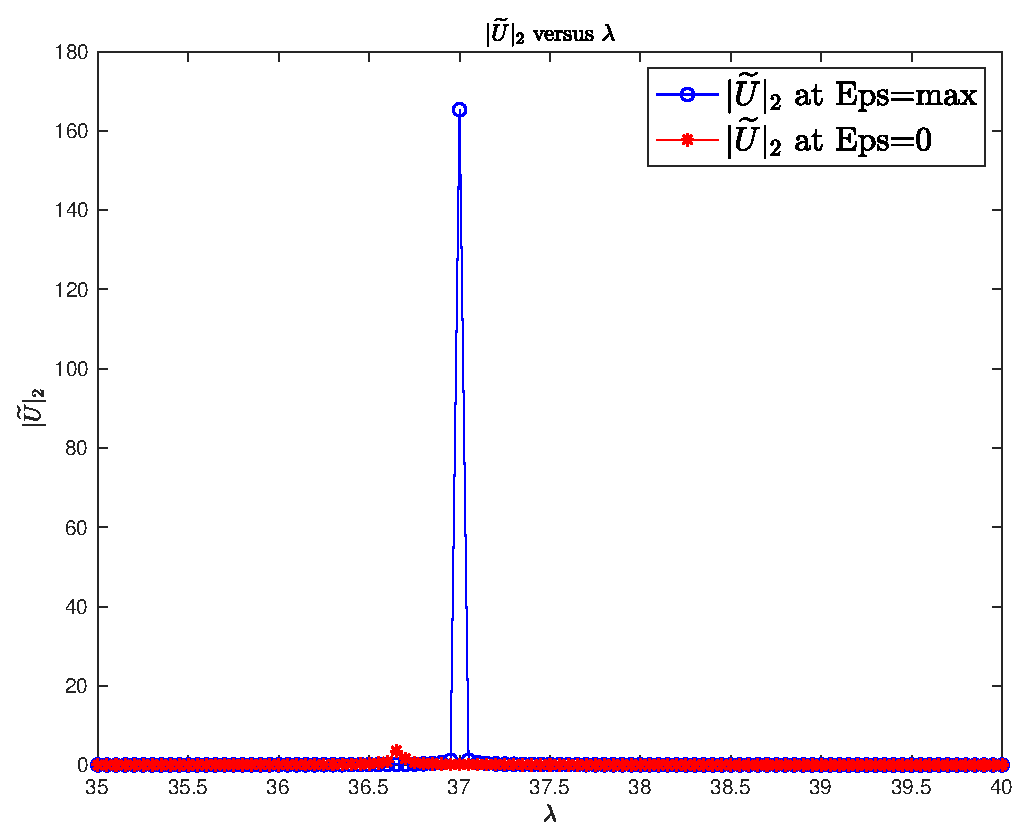
\includegraphics[width=0.35\textwidth]
		{fig_LGSPR_GU_shift_cos2_gbar25_VACUUM.pdf}}
	\quad
	\subfigure 
	{\includegraphics[width=0.35\textwidth]
		{fig_LGSPR_GW_shift_cos2_gbar25_VACUUM.pdf}}
	\\
	\subfigure
	{\includegraphics[width=0.35\textwidth]
		{fig_LGSPR_GU_shift_cos2_gbar50_VACUUM.pdf}}
	\quad
	\subfigure
	{\includegraphics[width=0.35\textwidth]
		{fig_LGSPR_GW_shift_cos2_gbar50_VACUUM.pdf}}
	\\
	\subfigure 
	{\includegraphics[width=0.35\textwidth]
		{fig_LGSPR_GU_shift_cos2_gbar500_VACUUM.pdf}}
	\quad
	\subfigure 
	{\includegraphics[width=0.35\textwidth]
		{fig_LGSPR_GW_shift_cos2_gbar500_VACUUM.pdf}}
	\\
	\subfigure 
	{\includegraphics[width=0.35\textwidth]
		{fig_LGSPR_GU_shift_cos2_gbar1000_VACUUM.pdf}}
	\quad
	\subfigure 
	{\includegraphics[width=0.35\textwidth]
		{fig_LGSPR_GW_shift_cos2_gbar1000_VACUUM.pdf}}
\end{figure}

\noindent\textbf{\large LGSPR  with (ALMA), vacuum and vacuum, $\cos(4\theta)$, $\bar{g} = 0.025, 0.05, 0.5, 1$}
\begin{figure}[H]
	\centering
	\subfigure
	{\includegraphics[width=0.35\textwidth]
		{fig_LGSPR_GU_shift_cos4_gbar25_VACUUM.pdf}}
	\quad
	\subfigure 
	{\includegraphics[width=0.35\textwidth]
		{fig_LGSPR_GW_shift_cos4_gbar25_VACUUM.pdf}}
	\\
	\subfigure
	{\includegraphics[width=0.35\textwidth]
		{fig_LGSPR_GU_shift_cos4_gbar50_VACUUM.pdf}}
	\quad
	\subfigure
	{\includegraphics[width=0.35\textwidth]
		{fig_LGSPR_GW_shift_cos4_gbar50_VACUUM.pdf}}
	\\
	\subfigure 
	{\includegraphics[width=0.35\textwidth]
		{fig_LGSPR_GU_shift_cos4_gbar500_VACUUM.pdf}}
	\quad
	\subfigure 
	{\includegraphics[width=0.35\textwidth]
		{fig_LGSPR_GW_shift_cos4_gbar500_VACUUM.pdf}}
	\\
	\subfigure 
	{\includegraphics[width=0.35\textwidth]
		{fig_LGSPR_GU_shift_cos4_gbar1000_VACUUM.pdf}}
	\quad
	\subfigure 
	{\includegraphics[width=0.35\textwidth]
		{fig_LGSPR_GW_shift_cos4_gbar1000_VACUUM.pdf}}
\end{figure}

\noindent\textbf{\large LGSPR  with (ALMA), vacuum and vacuum, $\cos(4\theta)$, $\bar{g}=1$, $\lambda=35 \to 45$}
\begin{figure}[H]
	\centering
	\subfigure 
	{\includegraphics[width=0.35\textwidth]
		{fig_LGSPR_GU_shift_cos4_gbar1000_VACUUM_45.pdf}}
	\quad
	\subfigure 
	{\includegraphics[width=0.35\textwidth]
		{fig_LGSPR_GW_shift_cos4_gbar1000_VACUUM_45.pdf}}
\end{figure}

\newpage
\noindent\textbf{\large LGSPR  with (BFPV), vacuum and vacuum, $\exp(\cos)$, $\bar{g} = 0.0025, 0.05, 0.5, 1$}
\begin{figure}[H]
	\centering
	\subfigure
	{\includegraphics[width=0.35\textwidth]
		{fig_LGSPR_GU_shift_expcos_gbar25_VACUUM_BFPV.pdf}}
	\quad
	\subfigure 
	{\includegraphics[width=0.35\textwidth]
		{fig_LGSPR_GW_shift_expcos_gbar25_VACUUM_BFPV.pdf}}
	\\
	\subfigure
	{\includegraphics[width=0.35\textwidth]
		{fig_LGSPR_GU_shift_expcos_gbar50_VACUUM_BFPV.pdf}}
	\quad
	\subfigure
	{\includegraphics[width=0.35\textwidth]
		{fig_LGSPR_GW_shift_expcos_gbar50_VACUUM_BFPV.pdf}}
	\\
	\subfigure 
	{\includegraphics[width=0.35\textwidth]
		{fig_LGSPR_GU_shift_expcos_gbar500_VACUUM_BFPV.pdf}}
	\quad
	\subfigure 
	{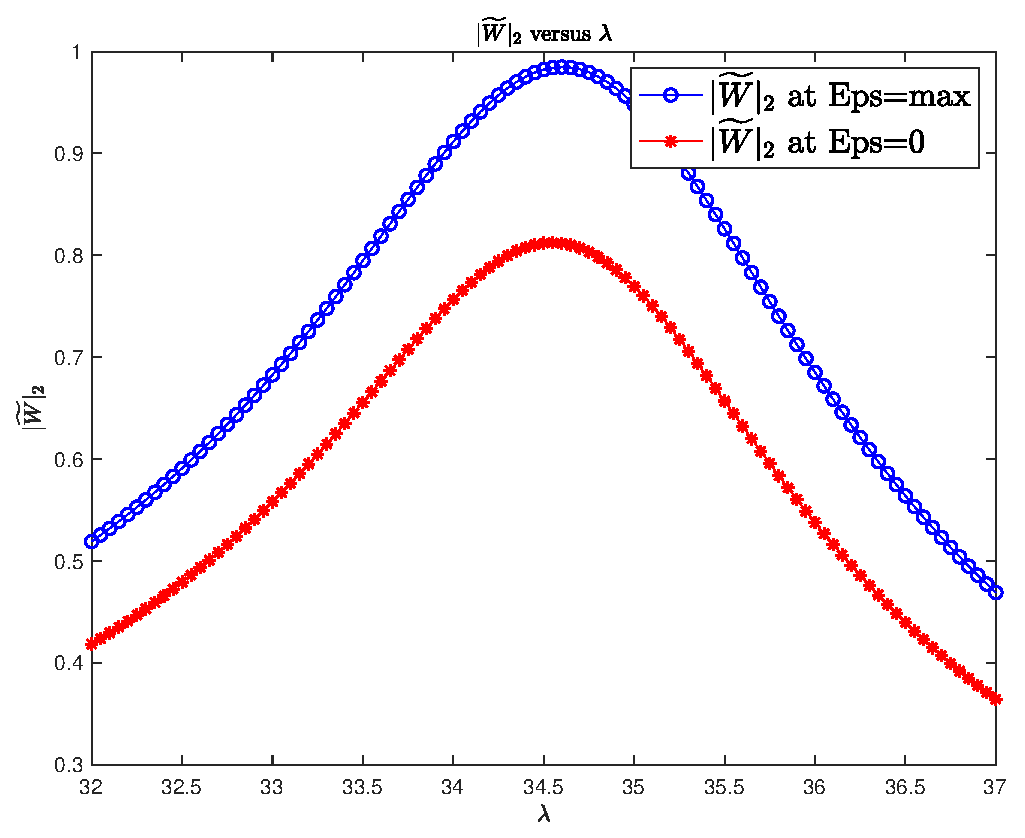
\includegraphics[width=0.35\textwidth]
		{fig_LGSPR_GW_shift_expcos_gbar500_VACUUM_BFPV.pdf}}
	\\
	\subfigure 
	{\includegraphics[width=0.35\textwidth]
		{fig_LGSPR_GU_shift_expcos_gbar1000_VACUUM_BFPV.pdf}}
	\quad
	\subfigure 
	{\includegraphics[width=0.35\textwidth]
		{fig_LGSPR_GW_shift_expcos_gbar1000_VACUUM_BFPV.pdf}}
\end{figure}

\noindent\textbf{\large LGSPR  with (BFPV), vacuum and vacuum,\quad $\exp(\cos)$, \quad $\lambda=34 \to 40$, \quad $\bar{g} =2$}
\begin{figure}[H]
	\centering
	\subfigure 
	{\includegraphics[width=0.35\textwidth]
		{fig_LGSPR_GU_shift_expcos_gbar2000_VACUUM_BFPV.pdf}}
	\quad
	\subfigure 
	{\includegraphics[width=0.35\textwidth]
		{fig_LGSPR_GW_shift_expcos_gbar2000_VACUUM_BFPV.pdf}}
\end{figure}

\newpage
\noindent\textbf{\large LGSPR  with (BFPV), vacuum and vacuum, $\cos(2\theta)$, $\bar{g} = 0.025, 0.05, 0.5, 1$}
\begin{figure}[H]
	\centering
	\subfigure
	{\includegraphics[width=0.35\textwidth]
		{fig_LGSPR_GU_shift_cos2_gbar25_VACUUM_BFPV.pdf}}
	\quad
	\subfigure 
	{\includegraphics[width=0.35\textwidth]
		{fig_LGSPR_GW_shift_cos2_gbar25_VACUUM_BFPV.pdf}}
	\\
	\subfigure
	{\includegraphics[width=0.35\textwidth]
		{fig_LGSPR_GU_shift_cos2_gbar50_VACUUM_BFPV.pdf}}
	\quad
	\subfigure
	{\includegraphics[width=0.35\textwidth]
		{fig_LGSPR_GW_shift_cos2_gbar50_VACUUM_BFPV.pdf}}
	\\
	\subfigure 
	{\includegraphics[width=0.35\textwidth]
		{fig_LGSPR_GU_shift_cos2_gbar500_VACUUM_BFPV.pdf}}
	\quad
	\subfigure 
	{\includegraphics[width=0.35\textwidth]
		{fig_LGSPR_GW_shift_cos2_gbar500_VACUUM_BFPV.pdf}}
	\\
	\subfigure 
	{\includegraphics[width=0.35\textwidth]
		{fig_LGSPR_GU_shift_cos2_gbar1000_VACUUM_BFPV.pdf}}
	\quad
	\subfigure 
	{\includegraphics[width=0.35\textwidth]
		{fig_LGSPR_GW_shift_cos2_gbar1000_VACUUM_BFPV.pdf}}
\end{figure}

\newpage
\noindent\textbf{\large LGSPR  with (BFPV), vacuum and vacuum, $\cos(4\theta)$, $\bar{g} = 0.025, 0.05, 0.5, 1$}
\begin{figure}[H]
	\centering
	\subfigure
	{\includegraphics[width=0.35\textwidth]
		{fig_LGSPR_GU_shift_cos4_gbar25_VACUUM_BFPV.pdf}}
	\quad
	\subfigure 
	{\includegraphics[width=0.35\textwidth]
		{fig_LGSPR_GW_shift_cos4_gbar25_VACUUM_BFPV.pdf}}
	\\
	\subfigure
	{\includegraphics[width=0.35\textwidth]
		{fig_LGSPR_GU_shift_cos4_gbar50_VACUUM_BFPV.pdf}}
	\quad
	\subfigure
	{\includegraphics[width=0.35\textwidth]
		{fig_LGSPR_GW_shift_cos4_gbar50_VACUUM_BFPV.pdf}}
	\\
	\subfigure 
	{\includegraphics[width=0.35\textwidth]
		{fig_LGSPR_GU_shift_cos4_gbar500_VACUUM_BFPV.pdf}}
	\quad
	\subfigure 
	{\includegraphics[width=0.35\textwidth]
		{fig_LGSPR_GW_shift_cos4_gbar500_VACUUM_BFPV.pdf}}
	\\
	\subfigure 
	{\includegraphics[width=0.35\textwidth]
		{fig_LGSPR_GU_shift_cos4_gbar1000_VACUUM_BFPV.pdf}}
	\quad
	\subfigure 
	{\includegraphics[width=0.35\textwidth]
		{fig_LGSPR_GW_shift_cos4_gbar1000_VACUUM_BFPV.pdf}}
\end{figure}

\noindent\textbf{\large LGSPR  with (BFPV), vacuum and vacuum, $\cos(4\theta)$, $\bar{g} = 1$, $\lambda=34 \to 40$}
\begin{figure}[H]
	\centering
	\subfigure 
	{\includegraphics[width=0.35\textwidth]
		{fig_LGSPR_GU_shift_cos4_gbar1000_VACUUM_BFPV_1.pdf}}
	\quad
	\subfigure 
	{\includegraphics[width=0.35\textwidth]
		{fig_LGSPR_GW_shift_cos4_gbar1000_VACUUM_BFPV_1.pdf}}
\end{figure}


\end{document}

